\section{Differentials, coordinate transformations, 
unisolvence and conformity of Prismatic Finite Elements}
\label{auxlabel110}
The motivation of the following exposition  is to extend and complete
what is said about coordinate transformations in~\cite{ciarlet},~\cite{gh99} and
Section 3.9 of~\cite{monk}.

We want the same setting to build Finite Elements on 
arbitrary contiguous prisms
belonging to a fixed mesh, all of them being an affine 
image of the reference prism.
In order to do so we transform the set $\hat{E}$ and show how to
pull--back and forward the scalars and fields in the 
discrete local spaces and the corresponding 
degrees of freedom.
%===============
%exactly as we are told by the 
%push-forward
%transformations~(\ref{push-forward}). 
%===============
Consider the application $\hat{\bx}\longmapsto{\bx} = 
F_E(\hat{\bx})$, where 
\begin{IEEEeqnarray}{rCl} \label{aux_label8}       
  F_E\hat\bx &= &M_E\hat{\bx} + \bx_0 
\end{IEEEeqnarray}
for an invertible matrix $M_E$,
that transforms
$\hat{E}$ onto an element $E$ of the mesh.

A scalar function $\hat{p} \in H^1(\hat{E})$ is transformed into a 
scalar function $p$ on $E$ with
\begin{IEEEeqnarray}{rCl}
    \label{transfEscalar} p\circ F_E & = & \hat{p}.
\end{IEEEeqnarray}
As it holds (cfr.~\cite{ciarlet})
\begin{IEEEeqnarray}{rCl} \label{aux_label4}
  \nabla p = M^{-t}\hat{\nabla} \hat{p} \circ F_E^{-1}\mbox{,}
\end{IEEEeqnarray}
then it results 
$p \in H^1(E)$. Gradients are taken with respect to the local coordinates
of $E$ and $\hat{E}$ in each case. The same will apply for every finite element
and for $\dv$ and $\curl$.

Now let $\hat{\bu} \in H(\bcurl, \hat{E})$. We want to assign to it a function
$\bu$ on $E$. As for $\hat{p}$ and $p$ as before it holds
$\nabla p \in H(\bcurl, E)$ and $\hat{\nabla} \hat{p} \in H(\bcurl, \hat{E})$,
equality~(\ref{aux_label4}) suggests the following transformation.
\begin{IEEEeqnarray}{rCl}
    \label{transfHcurl} \bu\circ F_E & = & M_E^{-t}\hat{\bu}.
\end{IEEEeqnarray} 
With this definition we have $\bu\in H(\bcurl, E)$ and also
\begin{IEEEeqnarray}{rCl}
    \label{transfCurl} (\curl\bu)\circ F_E & = & 
    \frac{1}{\det M_E} M_E (\curl\hat{\bu})\mbox{,}
\end{IEEEeqnarray}
(cfr. Lemma 3.57, page 77 and Corollary 3.58 in~\cite{monk}). For the important
example, needed in anisotropic analysis, with
\[
 M_E = \diag{h_1}{h_2}{h_3}
\]
it holds
\begin{IEEEeqnarray}{rCl}\label{aux_label29}
  \bh^{\balpha}({\partial}^{\balpha} \bu)\circ F_E & = & 
    M_E^{-t}\hat{\partial}^{\balpha} \hat\bu 
\end{IEEEeqnarray}
that is,
\begin{IEEEeqnarray}{rCl}
  \bh^{\balpha}({\partial}^{\balpha} \bu)\,\hat{} & = & 
    \hat{\partial}^{\balpha} \hat\bu. 
\end{IEEEeqnarray}
Now we proceed in the same way for $H(\Div)$. The relation 
$\hat\bu\in H(\bcurl,\hat E)$ implies $\curl\hat\bu\in H(\Div, \hat E)$
so~(\ref{transfCurl}) shows that to transform $\hat\bu\in H(\Div,\hat E)$
into $\bu\in H(\Div,E)$ we must do it via
\begin{IEEEeqnarray}{rCl}\label{transfDiv}
	\bu\circ F_E & = & \frac{1}{\det M_E}M_E\hat\bu.
\end{IEEEeqnarray}
If $\bu$ and $\hat\bu$ are related
by~(\ref{transfDiv}), then with a $\mathcal{D}(E)$ density argument we get 
\begin{IEEEeqnarray}{rCl} %% By Lemma 3.59 in~\cite{monk}
  \label{derivadaPiola} (\dv\,\bu)\circ F_E & = & (\det M_E)^{-1}\dv\,\hat\bu.
\end{IEEEeqnarray}
and hence $\bu\in H(\Div,E)$ if and only if $\hat\bu\in H(\Div,\hat E)$.

Normals and tangents are transformed as follows (cfr. page 265 of~\cite{giraultRaviart}).
Let $\hat{\bn}$ be the unit outward normal to $\hat E$.
If $\hat\bx\in\partial \hat{E}$ and $\bn$ is defined by
\begin{IEEEeqnarray}{rCl} \label{aux_label9}
  \bn(F_E\hat\bx)&=&
    \frac{M_E^{-t}\hat{\bn}(\hat\bx)}{\|M_E^{-t}\hat{\bn}(\hat\bx)\|}\mbox{,}
\end{IEEEeqnarray} 
then $\bn$ is a unit normal to $E$. Second, let $\hat\btau$ be any
unit vector tangent to $\partial{\hat{E}}$ at $\hat\bx$. If $\btau$ is
given by
\begin{IEEEeqnarray}{rCl} \label{aux_label10}
  \btau(F_E\hat\bx)&=&
    \frac{M_E\hat{\btau}(\hat\bx)}{\|M_E\hat{\btau}(\hat\bx)\|}\mbox{,}
\end{IEEEeqnarray}
then $\btau$ is a unit vector tangent to $\partial E$ at $F_E\hat\bx$.
Surface differentials are changed in the following way.
\begin{IEEEeqnarray}{rCl} \label{surface_diffs}
    dS & = & \|M_E^{-t}\hat\bn\|\,|\det M_E|\,d\hat{S}.
\end{IEEEeqnarray}
%======================================================================
% With~(\ref{transfDiv})
% \begin{IEEEeqnarray*}{rCl}
%    \|\hat{\textbf{v}}\|^2_{L^2(\hat{E})}
%    &=& \sum_{1\leqslant i\leqslant 3}\|\hat{v}_i\|^2_{0,\hat{E}}\\[7pt]
%    &=& \sum_{1\leqslant i\leqslant 3}\frac{h_jh_k}{h_i}\,\|v_i\|^2_{0,K};\\[7pt]
%    \|\hat{v}_i\|^2_{0,\hat{E}}&=&\frac{h_jh_k}{h_i}\,\|v_i\|^2_{0,K}
% \end{IEEEeqnarray*}
% where $\{i,j,k\} = \{1,2,3\}$.
%======================================================================
%=================================================================
%\begin{lemma} For all $\tilde{\boldsymbol{\sigma}} \in H(\Divg, \tilde{K})$,
%$\boldsymbol{\sigma}$ results in
%$H(\Divg, K)$ and in fact
%\[
%    {div}\,\boldsymbol{\sigma}({\bx}) =
%        \frac{1}{\det DF}\,\tilde{{div}}\,\tilde{\boldsymbol{\sigma}}(\tilde{{\bx}}).
%\]
%\end{lemma}
%\begin{proof}
%Observe that
%\begin{IEEEeqnarray*}{rCl}
%    trace(A\cdot B\cdot A^{-1}) &=& trace(B)\\
%    \label{Piola}\yesnumber\boldsymbol{\sigma} \circ F & = & \frac{1}{\det(A)} A\,\tilde{\boldsymbol{\sigma}}\\
%    \label{derivadaPiola}\yesnumber D\tilde{\boldsymbol{\sigma}}(\tilde{\bx}) & = &
%        \det(A)\,A^{-1}\,D\boldsymbol{\sigma} (F(\tilde{\bx})) \,A.
%\end{IEEEeqnarray*}
%Then
%\begin{IEEEeqnarray*}{rCl}
%    \text{div}\,\boldsymbol{\sigma}(\bx) & = & trace(D\boldsymbol{\sigma} (\bx))\\
%                                        & = & \frac{1}{\det(A)}\,trace(A\,\tilde{D}\tilde{\boldsymbol{\sigma}} (F^{-1}(\bx))\,A^{-1})\\
%                                        & = & \frac{1}{\det(A)}\,\tilde{\text{div}}\,\tilde{\boldsymbol{\sigma}}(\tilde{\bx}).   
%\end{IEEEeqnarray*}
%\end{proof}
%=================================================================

First a key result that establishes a relation between the interpolation
operators. It will used as an important step in the proof of the stability of the
edge element as well as in the proof of the stability of the face elements.
\begin{remark} In the reference~\cite{monk}, Lemma 5.40 in page 135 and the first Paragraph of Section 5.7 
in page 149 state the following facts.
  
Take the interpolation operator $\bw_{\hat E}$ of Definition~\ref{aux_label90}, 
the operator $\br_{\hat E}$ of Definition~\ref{defi_face_element}
and set $\pi^{\perp}_{\hat E}$ as
the $L^2$--orthogonal projection onto $P_k(\hat{E})$, then 
\begin{enumerate}
  \item 
For all sufficiently smooth $\hat\bu$ such that the interpolants
$\wku$ and $\br_{\hat E}\,\curl\hat\bu$ are both defined, then
\begin{IEEEeqnarray}{rCl}
\label{curl_commutativity}
  \curl\bw_{\hat E}\hat\bu &=& \br_{\hat E}\,\curl\hat\bu.
\end{IEEEeqnarray}
  \item 
For all sufficiently smooth $\hat\bu$ such that the interpolants
$\br_{\hat E}\hat\bu$ and $\pi^{\perp}_{\hat E}\,\dv\hat\bu$ are both  defined, then
\begin{IEEEeqnarray}{rCl}
\label{div_commutativity}
  \dv\,\rku & = & \pi^{\perp}_{\hat E}\,\dv\,\hat\bu.
\end{IEEEeqnarray}
\end{enumerate}
\end{remark}
%=============================================================
% \begin{proof}
% Vamos a usar la siguiente versión superficial del Teorema de Stokes. Sea dado un dominio Lipschitz acotado 
% $S\subseteq\mathbb{R}^2$ con tangente unitaria $\boldsymbol{\tau}$ al borde $\partial S$. Para 
% $\bu \in \mathcal{C}^1(\bar{S})^2 $ y $\phi \in \mathcal{C}^1(\bar{S})$ tenemos
% \begin{IEEEeqnarray}{rCl}
%     \int\limits_S \bu d\gamma & = &   %% HACER SEGUIR ACA
% \end{IEEEeqnarray}
% \end{proof}
%=============================================================
\noindent The last result can be expressed saying that the following diagram commutes:
\begin{center}
        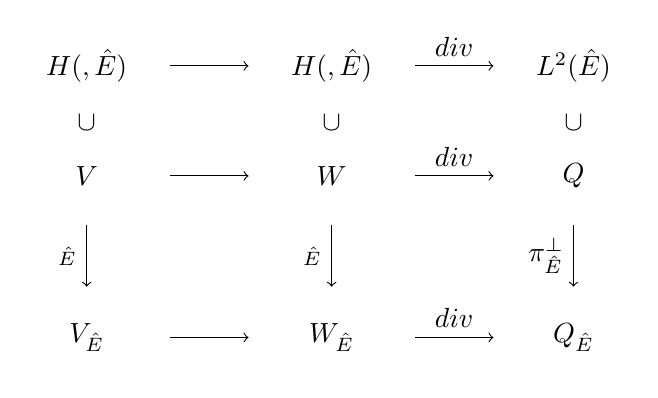
\begin{tikzpicture}[point/.style={circle, inner sep=0pt, minimum size=2pt,fill=red}]
            \matrix[column sep = 1.82mm, row sep = 1.1mm, ampersand replacement = \&] {
             \node {$\text{H}(\bcurl,\hat E)$};  
              \& \node (n0) {};
              \& \node      {};
              \& \node (n1) {};
              \& \node (n2) {};
              \& \node {$\text{H}(\Div, \hat E)$}; 
              \& \node (r1c7) {};
              \& \node {};
              \& \node {};
              \& \node (r1c10) {};
              \& \node {$L^2(\hat E)$};\\
             \node (n3) {}; \&\&\&\&\& \node (n5)   {};
              \& \node (r2c7) {};
              \& \node {};
              \& \node {};
              \& \node {};
              \& \node (r2c11) {};\\
             \node (n4) {}; \&\&\&\&\& \node (n6)   {};
              \& \node (r3c7) {};
              \& \node {};
              \& \node {};
              \& \node {};
              \& \node (r3c11) {};\\
             \node (v)  {$V$}; \&\node(fromV){};\&\&\&\node(toW){};\& \node (w) {$W$};
              \& \node (r4c7) {};
              \& \node {};
              \& \node {};
              \& \node (r4c10) {};
              \& \node {$Q$};\\
             \node (n7) {}; \&\&\&\&\& \node (n8)   {};
              \& \node {};
              \& \node {};
              \& \node {};
              \& \node {};
              \& \node (r5c11) {};\\
             \node      {}; \&\&\&\&\& \node        {}; 
              \& \node {};
              \& \node {};
              \& \node {};
              \& \node {};
              \& \node {};\\
             \node      {}; \&\&\&\&\& \node        {}; 
              \& \node {};
              \& \node {};
              \& \node {};
              \& \node {};
              \& \node {};\\
             \node (n11)    {}; \&\&\&\&\& \node (n12) {};
              \& \node {};
              \& \node {};
              \& \node {};
              \& \node {};
              \& \node (r8c11) {};\\
             \node {$V_{\hat E} $};                                 
              \& \node (n13) {};
              \& \node       {};
              \& \node (n14) {};
              \& \node (n15) {};
              \& \node {$W_{\hat E} $}; 
              \& \node (r9c7) {};
              \& \node {};
              \& \node {};
              \& \node (r9c10) {};
              \& \node {$Q_{\hat E}$};\\
             };
            \draw[->] (n0) to node[above] {$\bcurl$} (n2); 
            \draw[->] (fromV) to node[above] {$\bcurl$} (toW); 
            \draw[white] (n3) to node {{\color{black}$\cup$}} (n4);
            \draw[white] (n5) to node {{\color{black}$\cup$}} (n6);
            \draw[->] (n7) to node[left] {$\bw_{\hat E}$} (n11); 
            \draw[->] (n8) to node[left] {$\br_{\hat E}$} (n12); 
            \draw[->] (n13) to node[above] {$\bcurl$} (n15); 
            \draw[->] (r1c7) to node[above] {$\text{div}$} (r1c10);
            \draw[->] (r4c7) to node[above] {$\text{div}$} (r4c10);
            \draw[->] (r9c7) to node[above] {$\text{div}$} (r9c10);
            %\draw[white] (r2c7) to node {{\color{black}$\cup$}} (r3c7);
            \draw[white] (r2c11) to node {{\color{black}$\cup$}} (r3c11);
            \draw[->] (r5c11) to node[left] {$\pi^{\perp}_{\hat E}$} (r8c11);
        \end{tikzpicture}
    \end{center}
where $V_{\hat E}$, $W_{\hat E}$ and $Q_{\hat E}$ are the 
spaces~(\ref{spaceFEprismHcurl}),~(\ref{prismaticSpace})
and $P_0(\hat E)$ respectively.
\begin{defi} 
Suppose $\Omega$ is the union of two elements $E_1$ and $E_2$ with a common face $f$, 
we say that the family of unisolvent Finite Elements $(E, P_E, \Sigma)$ is conforming in 
some functional space $\mathbb{W}$
if, writing $\pi_1$, $\pi_2$
the interpolation operators determined by the degrees
of freedom $\Sigma_1$ and $\Sigma_2$, on $E_1$ and $E_2$, the field defined as
\begin{IEEEeqnarray*}{rCl}
  \bw & = &
    \begin{cases}
      \pi_1(\bu|_{E_1}), &\text{ on }E_1\\
      \pi_2(\bu|_{E_2}), &\text{ on }E_2      
    \end{cases}
\end{IEEEeqnarray*}
results in $\mathbb{W}(E_1\cup E_2)$.
\end{defi}
\begin{lemma} \label{aux_label7}
Let $\hat E$ be the reference prism~(\ref{defi_of_ref_prism}) and
let $P_{\hat E}$ be the space in~(\ref{spaceFEprismHcurl}), that is,
\begin{IEEEeqnarray*}{rCl}
  P_{\hat{E}} & = & R_k(\hat{x}_1,\hat{x}_2) \otimes P_k(\hat{x}_3) \times 
            P_k(\hat{x}_1,\hat{x}_2) \otimes P_{k-1}(\hat{x}_3).
\end{IEEEeqnarray*}
Provided the matrix $M_E$ is block--diagonal in the following manner
\begin{IEEEeqnarray*}{rCl}
  M_E & = & \blockdiag{m_{1,1}}{m_{1,2}}{m_{2,1}}{m_{2,2}}{m_{3,3}}\mbox{,}
\end{IEEEeqnarray*}
then $P_{\hat{E}}$ is invariant by transformation~(\ref{transfHcurl}).
\end{lemma}
\begin{proof}
  Starting with transformation~(\ref{transfHcurl}) take 
  $\hat{\bu}=(\hat u_1,\hat u_2,\hat u_3)'\in P_{\hat E}$
  and $\bu := (M_E^{-t}\hat{\bu})\circ F_E^{-1}$.
  Let 
  \[
    M_2 = \left(
    \begin{array}{cc}
      m_{1,1}  & m_{1,2}\\
      m_{2,1}  & m_{2,2} 
    \end{array}
    \right)
  \]
  and let $m_{i,j}^{(-1)}$ denote the coefficients of the inverse.
  By definition, 
  $(\hat u_1,\hat u_2)' = \hat{q}(\hat\bp + \hat{\boldsymbol{s}})$ for some
  $\hat\bp$, $\hat{\boldsymbol{s}}$ as in the spaces~(\ref{defSk}) and~(\ref{defRk}) and
  $\hat{q}\in P_{k}(\hat x_3).$ Using the blocks of $M_E$ and the tensor nature of
  $P_{\hat E}$,
  \begin{IEEEeqnarray*}{rCl}
    (u_1(\bx),u_2(\bx))' & = & (\hat{q}M_2^{-t}(\hat\bp + 
      \hat{\boldsymbol{s}}))(M_E^{-1}\bx - M_E^{-1}\bx_E)\\
    & = & \hat{q}(m_{3,3}^{(-1)}(x_3-x_{E,3}))(M_2^{-t}(\hat\bp + 
      \hat{\boldsymbol{s}}))(M_2^{-1}\bx - M_2^{-1}\bx_E).
  \end{IEEEeqnarray*}
  Now, $\hat{q}(m_{3,3}^{(-1)}(x_3-x_{E,3}))$ is a polynomial $q(x_3)$ with the
  same 
  degree as $\hat{q}$ is with respect to $\hat x_3$. Furthermore,
  as by Remark~\ref{aux_label6} $\hat{\boldsymbol{s}}$ has degree $\leqslant k-1$,
  expression $(M_2^{-t}(\hat\bp + \hat{\boldsymbol{s}}))(M_2^{-1}\bx - M_2^{-1}\bx_E)$
  can be seen as
  $M_2^{-t}(\bp(x_1,x_2) + \hat{\boldsymbol{s}}(M_2^{-1}\bx))$ with $\bp$
  having the expected degrees. And now
  \begin{IEEEeqnarray*}{rCcCl}
    M_2^{-t}\hat{\boldsymbol{s}}(M_2^{-1}\bx)\cdot(x_1,x_2)'
        &=& 
    \hat{\boldsymbol{s}}(M_2^{-1}(x_1,x_2)')\cdot M_2^{-1}(x_1,x_2)' &=& 0.
  \end{IEEEeqnarray*}
  The invariance of the third component of elements in $P_{\hat E}$ is
  an immediate consequence of the affine nature of the coordinate change.
\end{proof}
Now we are stating definitions and properties for the finite
element space in the case in which the prisms are not necessarily right, that
is, the matrix of the affine transformation from the reference element
needs no longer to be as in Lemma~\ref{aux_label7}. We are calling these prisms \emph{oblique}.
\begin{defi}\label{auxlabel415}
Let an oblique prism 
$E = F_E(\hat{E})$ be given as the affine image under
transformation~\eqref{aux_label8} from $\hat{E}$. Recall the reference space
$P_{\hat E}$ from~\eqref{spaceFEprismHcurl}. The local $H(\bcurl)$ finite element space is
defined as
\begin{IEEEeqnarray*}{rCl}
  P_E& = &\{M_E^{-t}\hat{\bu}\circ F_E^{-1}\,|\, \hat\bu\in P_{\hat E} \}.
\end{IEEEeqnarray*}
\end{defi}
\begin{lemma}\label{aux_label14}
Let a physical oblique prism $E = F_E(\hat{E})$ for $F_E$ as in~(\ref{aux_label8}).
Given $\hat\bu$ defined in $\hat{E}$ let $\bu$ in $E$ be determined by~(\ref{transfHcurl}), and
let $\hat\btau$, $\btau$, $\hat\bn$ and $\bn$ be tangents and normals to edges and
faces satisfying $F_E(\hat\be) = \be$ and $F_E(\hat{f}) = f$
in $\hat E$ and $E$, and 
related to each other by~(\ref{aux_label10}) and~(\ref{aux_label9}). Suppose
we define degrees of freedom of $\bu$ on $E$ as
\begin{IEEEeqnarray}{ll}
  \nonumber\varphi_{\be_i,p}\,(\bu) = 
  \int_{\be} q\,\bu \cdot d\balpha  
    &\quad  q\in P_{k-1}\mbox{,} \\
    \label{momentos1hcurlPhys}  
    &\quad  \mbox{ for each edge $\be$; }\\[8pt]
  \nonumber\varphi_{f,\bq}\,(\bu) =  
  \int_{f} \bu \cdot \bq_0\,
  dS\mbox{, } &\quad \bq_0 = (\det M_E\|M_E^{-t}\hat\bn\|)^{-1} M_E\,\hat{\bq}_T\\
  \nonumber&\quad \hat{\bq}_T := (\hat\bn\times\hat\bq)\times\hat\bn\\
  \label{momentos2hcurlPhys} 
  &\quad \mbox{$\hat\bq$ as in~(\ref{momentos2hcurl})--(\ref{momentos5hcurl})}.\\[8pt]
  \nonumber\varphi_{\br}(\bu) = 
  \int_{E} \bu \cdot \br \, d\bx\mbox{, }&\quad \br = (\det M_E)^{-1} M_E\,\hat\br \circ F_E^{-1}\\
  \label{momentos3hcurlPhys}
  &\quad \hat\br \in P_{k-2,k-2} \times P_{k-3,k-1}.
\end{IEEEeqnarray}
Provided $\det M_E > 0$, the degrees of freedom~(\ref{momentos1hcurlPhys})--(\ref{momentos3hcurlPhys})
are identical to the referential degrees of freedom~(\ref{momentos1hcurl})--(\ref{momentos6hcurl}).
\end{lemma}
\begin{remark}
  For this Lemma we don't need the matrix $M_E$ to be as in Lemma~\ref{aux_label7}, so
  it is more general. If the matrix $M_E$ is not block diagonal as we stated before, the local
  space in a physical prism element does not necessarily have the same structure as in the 
  reference prism. This is not a restriccion, since in our main Theorem and in our 
  applications we needed only right prisms.

\end{remark}
\begin{proof}[Proof of Lemma~\ref{aux_label14}]
  For the degrees of freedom over the edges take a parameterization
  $\hat{\boldsymbol{\alpha}}(t):I=[0,1]\to \hat\be$ such that
  \[
    \hat\btau = \frac{\stackrel{.}{\hat{\boldsymbol{\alpha}}}(t)}
    {\|\stackrel{.}{\hat{\boldsymbol{\alpha}}}(t)\,\|}.
  \]
  As a jacobian maps tangents into tangents,
  $\balpha(t) = M_E\,\hat{\balpha}(t) + \bx_E$ parameterizes
  $\be$. Then
  \begin{IEEEeqnarray*}{rCl}
    \int_{\be}(q\bu)\cdot d\boldsymbol{\alpha}
    &=&\int_{I}
    q\bu(F\hat{\boldsymbol{\alpha}}(t)))\cdot M_E
    \stackrel{.}{\hat{\boldsymbol{\alpha}}}(t)\,dt  \\[5pt]
    &=&\int_{I}
    \hat q(\hat{\boldsymbol{\alpha}}(t)) M_E^{-t}
    \hat\bu(\hat{\boldsymbol{\alpha}}(t))\cdot M_E\stackrel{.}{\hat{\boldsymbol{\alpha}}}(t)\,dt\\[5pt]
    &=&\int_{\hat\be}(\hat q\hat\bu)\cdot d\boldsymbol{\hat\alpha}.
  \end{IEEEeqnarray*}
  Continuing with the surface degrees of freedom, 
  \begin{IEEEeqnarray*}{rCl}
    \int_{\hat f} \hat\bv\times\hat\bn\cdot\hat\bq\times\hat\bn\,d\hat S 
    & = & \int_{\hat f} (\hat\bn\times\hat\bq)\times\hat\bn\cdot\hat\bu\,d\hat S \\
    & = & \int_{\hat f} \det M_E\|M_E^{-t}\hat\bn\| \bq_0 (F\hat\bx) \cdot \bu(F\hat \bx) d\hat S \\
    & = & \int_{ f} \bq_0 (\bx) \cdot \bu( \bx) d S
  \end{IEEEeqnarray*}
  Finally, for the volume degrees of freedom,
  \begin{IEEEeqnarray}{rCl}
    \int_{E}\bv\cdot\br\,d\bx
    & = & 
    \int_{\hat E}M_E^{-t}\hat\bv(F_E^{-1}\bx)\cdot
      (\det M_E)^{-1}M_E\hat\br(F_E^{-1}\bx)\,d\hat\bx.\\
    & = & 
    \int_{\hat E}\hat\bv(\hat\bx)\cdot\hat\br(\hat\bx)\,d\hat\bx.
  \end{IEEEeqnarray} 
\end{proof}
In the following corollary we complete Theorem 8 in page $75$ of~\cite{nedelec2}
which has only the case of the reference element.
\begin{corollary} The finite element in Definition~\ref{edgeelement} determines a family
of $H(\bcurl)$--conforming and unisolvent finite elements provided we use the degrees
of freedom transformations~(\ref{momentos1hcurlPhys}),~(\ref{momentos2hcurlPhys})
and~(\ref{momentos3hcurlPhys}).
\end{corollary}
\begin{proof}
  Transform the degrees of freedom from Lemma~\ref{aux_label14} back to $\hat E$
  and use unisolvence over the reference element.
\end{proof}
\begin{corollary}
 \label{aux_label26} 
  For any $\bu\in W^{1,p}(E)$ expressions~(\ref{momentos1hcurlPhys})--(\ref{momentos3hcurlPhys}) 
  determine a well defined $k$--th order local interpolate
  $\bw_E\,\bu$ defined as the unique finite element function in $P_E$ such that
  \begin{IEEEeqnarray}{lClc}
    \varphi_{\be,q}\,(\bu - \bw_E\,\bu) & = & 0 &
    \quad\mbox{for $\varphi_{\be,q}$ as in~(\ref{momentos1hcurlPhys})}\\
    \varphi_{f,\bq}\,(\bu - \bw_E\,\bu) & = & 0 &
    \quad\mbox{for $\varphi_{f,\bq}$ as in~(\ref{momentos2hcurlPhys})}\\
    \varphi_{\br}\,(\bu - \bw_E\,\bu) & = & 0 &
    \quad\mbox{for $\varphi_{\br}$ as in~(\ref{momentos3hcurlPhys})}.
  \end{IEEEeqnarray}
\end{corollary}
This will be used in the proof of local interpolation estimates.
\begin{lemma} Provided $\det M^{t} > 0$, the edge element interpolators satisfy
\begin{IEEEeqnarray}{rCl}\label{piTransformado}
    \wku(\hat{\bx}) & = & M^{t} \bw_E\bu(F_E(\hat{\bx}))
\end{IEEEeqnarray}
That is, the interpolator commutes with the coordinate change~(\ref{transfHcurl}).
\end{lemma}
\begin{proof} 
  By definition, for all degree of freeom 
  $\varphi$ in~(\ref{momentos1hcurlPhys})--(\ref{momentos3hcurlPhys}) it holds
  \[
    \varphi(\bu - \bw_E\bu) = 0.
  \]
  By the invariance of degrees of freedom
  proved in Lemma~\ref{aux_label14}, it follows
  \[
  \hat{\varphi}\left((\bu - \bw_E\bu){\,\hat{}\,}\right) = 
  \hat{\varphi}\left(\hat{\bu} - (\bw_E\bu){\,\hat{}\,}\right) = 0
  \]
  which implies $\wku = \hat{\bw}_E(\bw_E\bu){\,\hat{}}$\,.
  The space $P_{\hat E}$ was proven to be invariant under~(\ref{transfHcurl}), so
  $\wku = (\bw_E\bu){\,\hat{}}$\,.
\end{proof}
In the following paragraph we make all the previous exposition 
for the divergence finite elements.  
\begin{lemma}\label{aux_label13} Let $\hat E$ be the reference prism~(\ref{defi_of_ref_prism}) and
let $P_{\hat E}$ be the space in~(\ref{prismaticSpace}).
Provided the matrix $M_E$ is block--diagonal as in Lemma~\ref{aux_label7},
then $P_{\hat{E}}$ is invariant by transformation~(\ref{transfDiv}).
\end{lemma}
\begin{proof} The property follows with the same direct approach as 
Lemma~\ref{aux_label7} and in a much simpler case.
\end{proof}
\begin{defi}\label{auxlabel416}
Let an oblique prism 
$E = F_E(\hat{E})$ be given as the affine image under
transformation~\eqref{aux_label8} from $\hat{E}$. Recall the reference space
$P_{\hat E}$ from~\eqref{prismaticSpace}. The local $H(\Div)$ finite element space is
defined as
\begin{IEEEeqnarray*}{rCl}
  P_E& = &\left\{{\det M_E^{-1}} M_E\hat\bu \circ F_E^{-1} \,|\, \hat\bu\in P_{\hat E} \right\}.
\end{IEEEeqnarray*}
\end{defi}
\begin{lemma} \label{aux_label12}
Let an oblique prism $E = F_E(\hat{E})$ for $F_E$ as in~(\ref{aux_label8}).
Given $\hat\bu\in W^{1,1}(\hat E)$ let $\bu$ in $E$ be determined by~(\ref{transfDiv}), and
let $\hat\bn$ and $\bn$ be normals to faces satisfying $F_E(\hat{f}) = f$
in $\hat E$ and $E$, and 
related to each other by~(\ref{aux_label9}). Suppose
we define degrees of freedom of $\bu$ on $E$ as
\begin{IEEEeqnarray}{cCccl}
    \nonumber\rho_{ f,q}(\bv) & = & \int_{f} (\bv\cdot\bn)q\,dS 
        &\quad & \mbox{for } q = \hat{q}\circ F_E^{-1}, \hat{q} \in P_{k-1}(\hat{f})\mbox{,}\\
    \label{momentos1hdivPhys} 
    &&&\quad&\mbox{if $ \hat{f} =  \hat{f}_3$ or $ \hat{f}_4$;}\\[5pt]
    \nonumber
    \rho_{ f,q}(\bv) & = & \int_{f} (\bv\cdot\bn)q\,dS 
        &\quad & \mbox{for } q = \hat{q}\circ F_E^{-1}, \hat{q} \in Q_{k-1, k-1}(\hat f)\mbox{,}\\
    \label{momentos2hdivPhys}
    &&&\quad&\mbox{ if $ \hat{f} =  \hat{f}_1$, $ \hat{f}_2$ or $ \hat{f}_5$;}\\[5pt]
    \nonumber
    \rho_{ \br}(\bv) & = & \int_{{E}} \bv\cdot\br\,d\bx 
        &\quad& \mbox{for }\br = M_E^{-t}\hat\br\circ F_E^{-1}, \\
    \label{momentos3hdivPhys}
        &&&&\hat\br\in (P_{k-2,k-1})^2 \times P_{k-1,k-2}.
\end{IEEEeqnarray}
Provided $\det M_E > 0$, the degrees of freedom~(\ref{momentos1hdivPhys})--(\ref{momentos3hdivPhys})
are identical to the referential degrees of freedom~(\ref{momentos1hdiv})--(\ref{momentos4hdiv}).
\end{lemma}
\begin{proof}
  On one hand, by~(\ref{transfDiv}) and~(\ref{surface_diffs}),
  \begin{IEEEeqnarray*}{rCl}
    \int_{f} \bv\cdot\bn\bq\,d S & = & 
    \int_{f} (\det M_E)^{-1} \hat\bv(F_E^{-1}\bx)\cdot\|M_E^{-t}\hat\bn\|^{-1}\hat\bn\hat\bq(F_E^{-1}\bx)\,d S \\
    & = &\int_{\hat f} \hat\bv(\hat\bx)\cdot\hat\bn\hat\bq(\hat\bx)\,d\hat S.
  \end{IEEEeqnarray*}    
On the other hand,
  \begin{IEEEeqnarray}{rCcCl}
    \int_{E}\bv\cdot\br\,d\bx
    & = & 
    \int_{\hat E}M_E\hat\bv\cdot M_E^{-t}\hat\br\,d\hat\bx
    & = & 
    \int_{\hat E}\hat\bv\cdot\hat\br\,d\hat\bx.
  \end{IEEEeqnarray}
\end{proof}
\begin{lemma}\label{auxlabel414}
For a right prism $E$ let $P_E$ be the image of the space 
$P_{\hat E}$ of~\eqref{prismaticSpace} under transformation~\eqref{transfDiv}
for a block diagonal matrix $M_E$ as in Lemma~\ref{aux_label7}.
If $\bu\in P_{E}$ is such that all the
  degrees of freedom~(\ref{momentos1hdivPhys}) or~(\ref{momentos2hdivPhys}) vanish
  on the respective face $f$, then the normal component of $\bu$ 
  vanishes identically on that face $f$.
\end{lemma}
\begin{proof}
  This fact is stated in the proof of Theorem 4, page 66 of~\cite{nedelec2} 
  only for the reference prism. By transforming the degrees of freedom to 
  the faces of $\hat E$ and back to the faces of $E$ using Lemma~\ref{aux_label12}
  we get the result.
\end{proof}
\begin{lemma}Let $P_E$ be the space of Lemma~\ref{auxlabel414}.
  If $\bu\in P_{E}$ is such that all the
  degrees of freedom~(\ref{momentos1hdivPhys})--(\ref{momentos3hdivPhys}) vanish, 
  then $\bu$ vanishes identically on $E$.
\end{lemma}
\begin{proof}
  In the case of the reference prism $\hat E$, we refer to the proof of 
  Theorem 4 in page 66 of~\cite{nedelec2}. For the general case,
  by the invariance of the finite element space $P_{E}$ under
  the transformation~(\ref{transfDiv}) (see Lemma~\ref{aux_label13}) we have our result.
\end{proof}
\begin{corollary}
The finite element in Definition~\ref{defi_h_div_conforme} determines a family
of $H(\Div)$--conforming and unisolvent finite elements provided we use the degrees
of freedom transformations~(\ref{momentos1hdivPhys}),~(\ref{momentos2hdivPhys}) and~(\ref{momentos3hdivPhys}).
\end{corollary}
\begin{corollary}
  For any $\bv\in W^{1,1}(E)$ expressions 
  ~(\ref{momentos1hdivPhys})--(\ref{momentos3hdivPhys}) 
  determine a well defined local interpolate
  $\br_E\,\bu$ defined as the unique finite element function in $P_E$ such that
  \begin{IEEEeqnarray}{lClc}
    \rho_{f,\bq}\,(\bv - \br_E\,\bu) & = & 0 &
    \quad\mbox{for $\rho_{f,\bq}$ as in~(\ref{momentos1hdivPhys})
      and~(\ref{momentos2hdivPhys})}\\
    \rho_{\br}\,(\bv - \br_E\,\bu) & = & 0 &
    \quad\mbox{for $\rho_{\br}$ as in~(\ref{momentos3hdivPhys})}.
  \end{IEEEeqnarray}
\end{corollary}
The proof of the following important corollary  is
like the one of~(\ref{piTransformado}).
\begin{corollary}\label{aux_label17}
  Given $\bu \in W^{1,1}(E)$, then
  \begin{IEEEeqnarray}{rCl} \label{div_interp_commutes}
    \rku & = & \det M_E\,(M_E^{-1}\,\br_E\,\bu)\circ F_E\mbox{,}
  \end{IEEEeqnarray}
  that is, the $H(\text{div})$ interpolator commutes with the coordinate
  change~(\ref{transfDiv}).
\end{corollary}
\begin{remark}
  Unisolvence and conformity of the finite elements on tetrahedra mentioned in
  Section~\ref{sec:tetrahedralFEs}
  are proved in Sections 5.4 and 5.5 of~\cite{monk}.
\end{remark}
%===========================
% See Lemmas 5.32 and 5.34 in pages 130 and 131 of~\cite{monk}, where
% it is proved for tetrahedra. Exacly the same considerations about the degrees
% of freedom therein apply to prove the Lemma for prisms or pyramids.  
% Ver (3.79) (3.80) en monk: transf. de normales y tangentes.\\\\
%===========================